\begin{minipage}[t]{0,4\textwidth}
  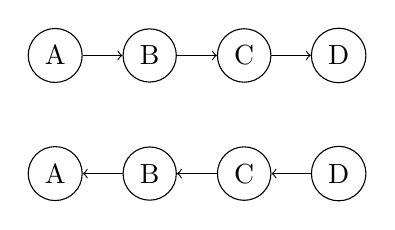
\begin{tikzpicture}
    \node[shape=circle,draw=black] (A) at (0,0) {A};
    \node[shape=circle,draw=black] (B) at (1.2,0) {B};
    \node[shape=circle,draw=black] (C) at (2.4,0) {C};
    \node[shape=circle,draw=black] (D) at (3.6,0) {D};
    \node[shape=circle,draw=black] (A1) at (0,-1.5) {A};
    \node[shape=circle,draw=black] (B1) at (1.2,-1.5) {B};
    \node[shape=circle,draw=black] (C1) at (2.4,-1.5) {C};
    \node[shape=circle,draw=black] (D1) at (3.6,-1.5) {D};
    \path [->](A) edge node {} (B);
    \path [->](B) edge node {} (C);
    \path [->](C) edge node {} (D);
    \path [<-](A1) edge node {} (B1);
    \path [<-](B1) edge node {} (C1);
    \path [<-](C1) edge node {} (D1);
  \end{tikzpicture}
\end{minipage}%

